% Copyright (C) 2022 by Maxime CHUPIN
% <chupin at ceremade.dauphine.fr>
% -------------------------------------------------------
%
% This work may be distributed and/or modified under the
% conditions of the LaTeX Project Public License, either version 1.3
% of this license or (at your option) any later version.
% The latest version of this license is in
%   http://www.latex-project.org/lppl.txt
% and version 1.3 or later is part of all distributions of LaTeX
% version 2005/12/01 or later.
%
%  Author: Maxime CHUPIN
%          chupin at ceremade.dauphine.fr
%
%  This work has the LPPL maintenance status "author-maintained".

\documentclass[10pt,aspectratio=169,english]{beamer}
\usepackage[charter]{mathdesign}
\usepackage{hologo}
\usepackage{luamesh}

\usepackage{babel}
\usepackage{pgfpages}
\usepackage{tcolorbox}
\usepackage{biblatex}
%\hypersetup{colorlinks=true}

\tcbuselibrary{listings,breakable}
\tcbuselibrary{documentation}
\tcbset{
  color command=AmurmapleRed,
  color environment=AmurmapleRed,
  color option=AmurmapleGreen
}
\usetheme[
%nogauge,
nomail,
delaunay,
%amurmapleblue
]{Amurmaple}

\lstset{
  numberstyle=\footnotesize\color{gray},
  keywordstyle=\ttfamily\bfseries\color{structure},
  basicstyle=\ttfamily\normalsize,
  commentstyle=\itshape\color{gray},
  stringstyle=\ttfamily,
  showstringspaces=false,
  language=[LaTeX]TeX,
  breaklines=true,
  breakindent=30pt,
  defaultdialect=[LaTeX]TeX,
  morekeywords={usetheme,definecolor, beamerbutton, beamerskipbutton,
    beamerreturnbutton, structure, alert, sectionpage, mail, webpage,
    collaboration, subtitle, institute, titlegraphic, sepframe, includegraphics,
    thanksframe, inserttitlegraphic, framesection, boxalert,appendix}
  % frame=tb
}


\newtcblisting{Code}{%
  arc=0pt,outer arc=0pt,
  colback=structure!3,
  colframe=structure,
  breakable,
  boxsep=0pt,left=5pt,right=5pt,top=5pt,bottom=5pt, bottomtitle =
  3pt, toptitle=3pt,
  boxrule=0pt,bottomrule=0.5pt,toprule=0.5pt, toprule at break =
  0pt, bottomrule at break = 0pt,
  listing options={breaklines,basicstyle=\ttfamily},listing only,
}

\newtcblisting{Exemple}{%
  arc=0pt,outer arc=0pt,
  colback=structure!3,
  colframe=structure,
  breakable,
  boxsep=0pt,left=3pt,right=3pt,top=2pt,bottom=2pt, bottomtitle =
  0pt, toptitle=0pt,
  boxrule=0pt,bottomrule=0.5pt,toprule=0.5pt, toprule at break =
  0pt, bottomrule at break = 0pt,
  listing options={breaklines,basicstyle=\ttfamily},
}

\newtcblisting{CodePreambule}{%
  arc=0pt,outer arc=0pt,
  colback=AmurmapleBlue!5,
  colframe=AmurmapleBlue,
  breakable,
  boxsep=0pt,left=5pt,right=5pt,top=5pt,bottom=5pt, bottomtitle =
  3pt, toptitle=3pt,
  boxrule=0pt,bottomrule=0.5pt,toprule=0.5pt, toprule at break =
  0pt, bottomrule at break = 0pt,
  enhanced,
  overlay  ={%
    \node[ minimum width=1cm,
      anchor=south east,yshift=-0cm,fill=AmurmapleBlue] at (frame.south east)
      {\itshape\color{white} preamble};
      % \node[ minimum width=1cm,
      % anchor=south east,yshift=-0cm,color=gray,opacity=0.7] at (frame.south east)
      % {\itshape\small préambule};
  },
  listing options={
    breaklines,
    basicstyle=\ttfamily,
  },listing only,
}




\title[Amurmaple documentation]{Amurmaple Beamer Theme}
\author[M.~Chupin]{Maxime Chupin}
\subtitle{documentation\quad v.1.0}
\institute[CNRS]{CNRS\\
University of Paris-Dauphine}
\date{Mai 28, 2022}
\titlegraphic{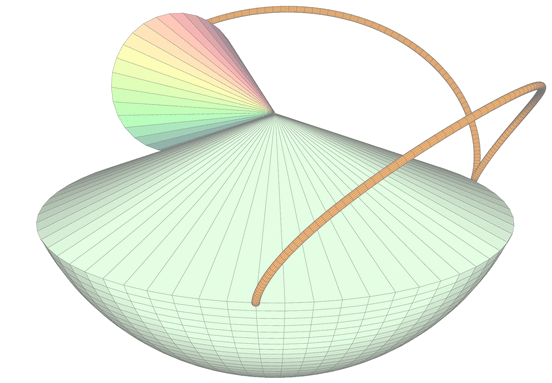
\includegraphics[width=4cm]{logo.png}}
\mail{chupin@ceremade.dauphine.fr}
\webpage{www.ceremade.dauphine.fr/~chupin/}
\collaboration{in collaboration with Beamer and \hologo{LaTeX3}}

\bibliography{biblio.bib}
\usefonttheme{serif}






\begin{document}

\maketitle

\sepframe[title={Table of contents}]
\section{Introduction}

\begin{frame}{Introduction}
\begin{information}
This Beamer theme is  a suitable theme for my use of Beamer in applied
mathematics research.

It meets my needs in my work. However, if you like this theme, and if you want
to ask for or make improvements, don't hesitate to write to me !

Obviously, we refer to the documentation of the Beamer class for details, and we
will assume in this little documentation that the reader is familiar with the
Beamer class.
\end{information}

\end{frame}


\section{How to use it}

\sepframe

\begin{frame}[fragile]{How to use Amurmaple theme}
  \begin{itemize}
  \item The Amurmaple beamer theme consists in the file
    \texttt{beamerthemeAmurmaple.sty} that you can put in your local
    \texttt{\~{}/texmf/tex/latex/contrib/beamer-contrib/themes/beamer-amurmaple}
    directory.
  \item Simply add in your preamble\footnote{Note that the listing environments
      of this document are not provided by Amurmaple theme.}
    \begin{CodePreambule}
\documentclass{beamer}
\usetheme{Amurmaple}
\end{CodePreambule}
\item This theme depends on the following packages:
  \begin{multicols}{2}
  \begin{itemize}
  \item \lstinline+tcolorbox+;
  \item \lstinline+multicol+;
  \item \lstinline+xparse+;
  \item \lstinline+xfp+;
  \item \lstinline+expl3+;
  \item \lstinline+iftex+.
  \end{itemize}
\end{multicols}
\end{itemize}
\end{frame}

\subsection{Theme Options}

\begin{frame}[fragile]{Theme Options}
  There are some options available :
  \begin{description}
  \item[nogauge:] that suppresses the gauge at the top of the vertical side bar
    of the current slide ;
  \item[nomail:] that suppresses the mail in the vertical side bar of
    the current slide ;
  \item[delaunay:] that produces a Delaunay mesh of random points in
    the ``structure'' slides (title, section, etc.). \alert{This option can only be
    used with \hologo{LuaLaTeX}} and depends on the
  package~\lstinline{luamesh}\footfullcite{Luamesh};
  \item[amurmapleblue:] that changes the main color (\lstinline+structure+) to a
    certain blue (see slide~\ref{sl:color}) ;
  \item[amurmaplegreen:] that changes the main color (\lstinline+structure+) to a
    certain green (see slide~\ref{sl:color});
  \end{description}
  For example, these slides are produced with the following call\footnote{We use
  the \texttt{charter} font family of \texttt{mathdesign}  with the serif Beamer theme.}:
  \begin{CodePreambule}
\usetheme[nomail,delaunay]{Amurmaple}
  \end{CodePreambule}
\end{frame}



\section{Classical Beamer Tools}
\sepframe
\subsection{Colors}

\begin{frame}[fragile, allowframebreaks]{Colors of the theme}
  This theme provides some colors :
  \begin{Code}
\definecolor{AmurmapleRed}{rgb}{0.6,0.,0.}
\definecolor{AmurmapleOrange}{RGB}{230,108,17}
\definecolor{AmurmapleBlue}{RGB}{55,119,231}
\definecolor{AmurmapleGreen}{rgb}{0.1,0.4,0.1}
\end{Code}

\textcolor{AmurmapleRed}{\lstinline+AmurmapleRed+} is used to redefine the \lstinline+structure+
Beamer color\footnote{So if you redefine the \lstinline+structure+ color, the Amurmaple
theme should change correctly.}, \textcolor{AmurmapleOrange}{\lstinline+AmurmapleOrange+} is used to redefine
the \lstinline+text alerted+ Beamer color, \textcolor{AmurmapleGreen}{\lstinline+AmurmapleGreen+} is
used for the math definition (see slide~\ref{sl:definition}) and for the
\lstinline+block title example+ Beamer color, and the
\textcolor{AmurmapleBlue}{\lstinline+AmurmapleBlue+} for the new environnement
\lstinline+information+ (see slide~\ref{sl:information}).
\framebreak

\framesection{Color Theme Option}\label{sl:color}

This theme provides two theme options to change the color settings:
\begin{description}
\item[amurmapleblue] that sets \texttt{AmurmapleBlue!80!black} as \texttt{structure}
  color ;
\item[amurmaplegreen] that sets \texttt{AmurmapleGreen!80!black} as \texttt{structure}
  color.
\end{description}
In fact, internally, four colors are defined: \lstinline+Amurmaple@structure+,
\lstinline+Amurmaple@alert+, \lstinline+Amurmaple@info+ and
\lstinline+Amurmaple@example+.

The color theme option is used as follow
\begin{Code}
  \usetheme[amurmapleblue]{amurmaple}
\end{Code}
\end{frame}

\subsection{Classical commands}

\begin{frame}[fragile]{Classical Beamer Commands}
  \framesubtitle{Customization}
  \framesection{Beamer buttons}
  \begin{Exemple}
\beamerbutton{Button}~\beamerskipbutton{Skip Button}~\beamerreturnbutton{Return}
\end{Exemple}
\framesection{Alert and structure commands}
\begin{Exemple}
\structure{Test structure} \alert{Test alert}
\end{Exemple}
\end{frame}

\begin{frame}[fragile]{Results of \texttt{$\backslash$tableofcontents}}
  \tableofcontents
\end{frame}

\subsection{Classical environnement}

\begin{frame}[allowframebreaks,fragile]{Classical Beamer environments}
  \framesection{Block environments}
  \begin{block}{Block}
    Test of the \lstinline+\begin{block}...\end{block}+ Beamer environment.
  \end{block}
  \begin{alertblock}{Alert Block}
    Test of the \lstinline+\begin{alertblock}...\end{alertblock}+ Beamer environment.
  \end{alertblock}
  \begin{exampleblock}{Example Block}
    Test of the \lstinline+\begin{exampleblock}...\end{exampleblock}+ Beamer environment.
  \end{exampleblock}

  \framebreak

\framesection{Abstract environment}

  \begin{abstract}
    This is the result of the \lstinline+\begin{abstract}...\end{abstract}+
    environment.
  \end{abstract}

  \framesection{Quotation environment}

  The environment \lstinline+\begin{quotation}[+\meta{author(s)}\lstinline+]...\end{quotation}+ has been
  redefined allowing an optional argument to provide the author(s) of the
  quotation.

  \begin{quotation}[Donald E. Knuth, \emph{The \TeX book}]
Gentle reader: This is a handbook about \TeX, a new typesetting system G
intended for the creation of beautiful books—and especially for books that
contain a lot of mathematics.
\end{quotation}

\framebreak
\framesection{Lists}

The style of the standard enumerate and itemize lists has been modified as you
can see below

\begin{multicols}{2}
  \begin{itemize}
\item Eggs
\item Plants
  \begin{itemize}
  \item Flowers
  \end{itemize}
\item Animals
\end{itemize}
\columnbreak
\begin{enumerate}
\item Eggs
\item Plants
\item Animals
  \begin{enumerate}
  \item Dogs
  \item Cats
  \end{enumerate}
\end{enumerate}
\end{multicols}
\end{frame}


\subsection{Section and Part Frames}

\newsavebox{\codebox}% To store any verbatim content
\begin{lrbox}{\codebox}
  \begin{Code}
\begin{frame}
\sectionpage
\end{frame}

%\begin{frame}
%\partpage
%\end{frame}
\end{Code}
\end{lrbox}

\begin{frame}[fragile]{Section and Part Frames}
  The standard \texttt{section page} and \texttt{part page} have been modified.

  The following code produce the next slide (the part slide is not generated
  because this document does not use part sectionning).

  \usebox{\codebox}

\end{frame}

\begin{frame}
\sectionpage
\end{frame}

\subsection{Maths}

\begin{frame}[fragile,allowframebreaks]{Maths environnement}
  \begin{itemize}
  \item \lstinline+\begin{theorem}+\oarg{Title of th. (optional)}\lstinline+...\end{theorem}+
    \begin{theorem}[Title of th. (optional)]
      There exists an infinite set.
    \end{theorem}
  \item \lstinline+\begin{example}...\end{example}+
    \begin{example}
      The set of natural numbers is infinite.
    \end{example}
  \item \lstinline+\begin{definition}+\oarg{Title of def. (optional)}\lstinline+...\end{definition}+\label{sl:definition}
    \begin{definition}[Title of def. (optional)]
      A simple definition.
    \end{definition}
    \framebreak
  \item \lstinline+\begin{corollary}+\oarg{Title of corollary (optional)}\lstinline+...\end{corollary}+
    \begin{corollary}[Title of corollary (optional)]
      A simple corollary.
    \end{corollary}
  \item \lstinline+\begin{proof}...\end{proof}+
    \begin{proof}
      This follows from the axiom of infinity.
    \end{proof}
  \end{itemize}
\end{frame}



\section{Title Page}

\sepframe

\begin{frame}[fragile,allowframebreaks]{Title Page}
  As shown in this document, the title page has been customized.
  In addition to the classic commands for making the title page, the Amurmaple
  theme provides new commands.

  The new commands are :
  \begin{itemize}
  \item \lstinline+\mail+\marg{mail}: that is used to provide the mail. Without the theme option
    \lstinline+nomail+, it is also added on the vertical side bar on the current
    slide.
  \item \lstinline+\webpage+\marg{webpage}: that is used to provide the personal webpage of
    the speaker (or the project website).
  \item \lstinline+\collaboration+\marg{collaboration(s)}: that is used to provide the collaborators
    for the presented work.
  \end{itemize}

  \framebreak

  Here the example used to generate this documentation.
  \begin{Code}
\title[Amurmaple documentation]{Amurmaple Beamer Theme}
\author[M.~Chupin]{Maxime Chupin}
\subtitle{documentation}
\institute[CNRS]{CNRS\\
University of Paris-Dauphine}
\date{Mai 08, 2022}
\titlegraphic{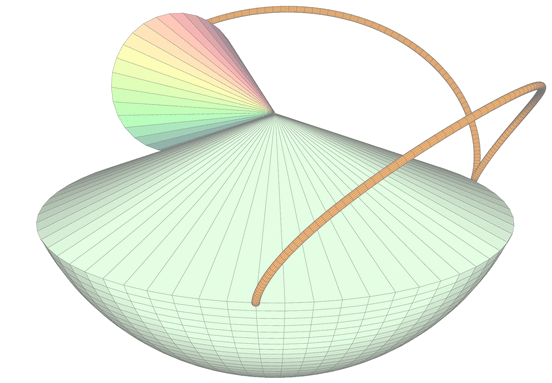
\includegraphics[width=4cm]{logo.png}}
\mail{chupin@ceremade.dauphine.fr}
\webpage{www.ceremade.dauphine.fr/~chupin/}
\collaboration{in collaboration with Beamer and \hologo{LaTeX3}}
\end{Code}

\end{frame}

\section{New Frame Commands}

\sepframe

\begin{frame}[fragile]{\texttt{sepframe} command}
\bigskip
\begin{docCommand}{sepframe}{\oarg{title=\meta{mytitle},image=\meta{my image}}}
The newcommand \lstinline+\sepframe+ is provided by the Amurmaple theme. This
command allows you to generate a slide in the manner of a section page but with
a slight improvement. In the red part below is generated the table of contents
(with depth 1).

Moreover, this command admits two optional arguments:
\begin{description}
\item[title:] this optional argument allows to modify the default title of the
  frame (which is the current section name) ;
\item[image:] this optional argument allows to add an image to the frame (no
  image by default).
\end{description}

\end{docCommand}



For exemple, we could use
\begin{Code}
\sepframe[title={My title},image={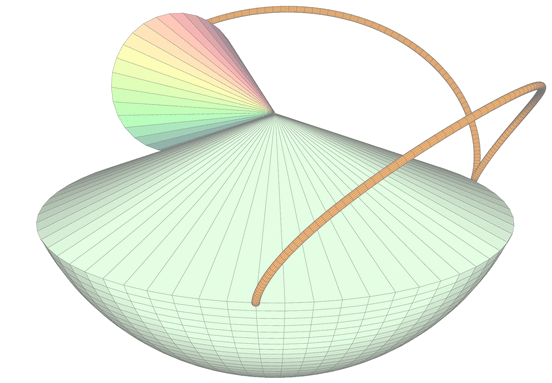
\includegraphics[width=5cm]{logo.png}}]
\end{Code}

The result is the next frame.
\end{frame}

\sepframe[title={My  title},image={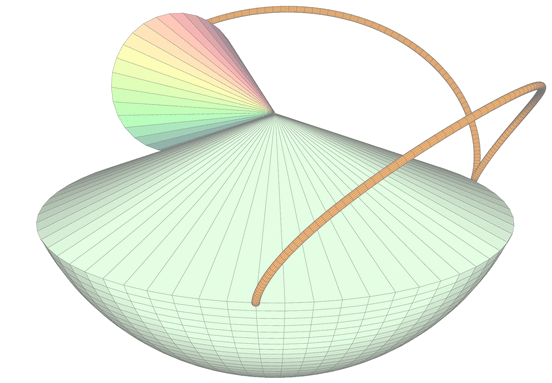
\includegraphics[width=5cm]{logo.png}}]

\begin{frame}[fragile]{\texttt{thanksframe} command}

  \begin{docCommand}{thanksframe}{\marg{thanking message}}
  The newcommand \lstinline+\thanksframe+ is provided by the Amurmaple
  theme. This command allows you to generate a slide  to thank the audience.
  The text written to thank is a mandatory argument (e.g. ``\emph{The end}'')
  and the optional argument allows to change the default image which is the
  \emph{title graphics} (\lstinline+\inserttitlegraphic+ exactly).
\end{docCommand}
The following code produces the next slide.
  \begin{Code}
\thanksframe{Merci beaucoup~!}
  \end{Code}
\end{frame}

\thanksframe{Merci beaucoup~!}

\section{New Commands and Environments}

\begin{frame}[fragile,allowframebreaks]{Some New Commands and Environments}
  The Amurmaple theme provides some other commands and environments.

  \framesection{New Commands}

  \begin{docCommand}{framesection}{\marg{text}}
    Command to add a section title inside a frame.

    The following example produced the previous frame sectioning \emph{New Commands}
    \begin{Code}
\framesection{New Commands}
\end{Code}
\end{docCommand}
\begin{docCommand}{boxalert}{\marg{text}}
Another \lstinline+\alert+ command with a colored box.
  \begin{Exemple}
\boxalert{This is another} command box to compare to \alert{this one}.
  \end{Exemple}
\end{docCommand}
\framebreak

\framesection{New Environments}
{\itshape \structure{Note:} Each environment provided by the Amurmaple theme uses
translations for title names. Hence, depending on the \texttt{babel} setting,
\emph{Remark} becomes \emph{Remarque, Bemerkung,}\dots}

\begin{docEnvironment}{information}{\oarg{changed title}}
 The Amurmaple theme provides an information environment.\label{sl:information}
  \begin{Code}
\begin{information}
  This is important information.
\end{information}
  \end{Code}
  \begin{information}
    This is an important information.
  \end{information}

  This environment has an optional argument to change the \emph{Information}
  title.
  \begin{Code}
\begin{information}[More information]
  Maybe more important information?
\end{information}
\end{Code}

\begin{information}[More information]
  Maybe more important information?
\end{information}
Because this environment is built with a \texttt{tcolorbox}, to use a footnote in it, you have to use \lstinline+\footnote[frame]{...}+.
\end{docEnvironment}

\begin{docEnvironment}{remark}{\oarg{title complement}}
The Amurmaple theme provides a remark environment with an optional
  argument to add a comment in the title (as for the theorem environment).
  \begin{Code}
\begin{remark}[Some complement]
  This is a capital remark.
\end{remark}
\end{Code}
\begin{remark}[Some complement]
  This is a capital remark.
\end{remark}

Because this environment is built with a \texttt{tcolorbox}, to use a footnote in it, you have to use \lstinline+\footnote[frame]{...}+.
\end{docEnvironment}

\end{frame}

\appendix

\section{Appendix}

\sepframe

\begin{frame}[fragile]{Appendix}
  In the appendix part of the document, (after the command
  \lstinline+\appendix+) the display is slightly modified as you
  can see in this slide. If the gauge exists, it disappears, the numbering
  of slides is reset and the display is in roman form.
\end{frame}


\thanksframe{The end!}



\end{document}

%%% Local Variables:
%%% mode: latex
%%% TeX-master: t
%%% End:
